\documentclass[conference]{IEEEtran}
\IEEEoverridecommandlockouts
% The preceding line is only needed to identify funding in the first footnote. If that is unneeded, please comment it out.
\usepackage{cite}
\usepackage{amsmath,amssymb,amsfonts}
\usepackage{graphicx}
\usepackage{textcomp}
\usepackage{xcolor}
\usepackage[hidelinks]{hyperref}
\usepackage{float}
\usepackage{booktabs}
\usepackage{array}
\usepackage{pgfplots}
\usepackage{placeins}
\usepackage{tikz}
\usetikzlibrary{positioning,calc,arrows.meta,shapes.geometric,fit,backgrounds}
\pgfplotsset{compat=1.18}
\def\BibTeX{{\rm B\kern-.05em{\sc i\kern-.025em b}\kern-.08em
    T\kern-.1667em\lower.7ex\hbox{E}\kern-.125emX}}
\newcommand{\cmark}{\ding{51}}
\usepackage{pifont}
\begin{document}


\title{
\fontsize{22}{25}\selectfont
CodeSheriff: Design and Development of an Agentic Security
Auditor for an SFI-Enabled Confidential CI/CD Execution
Layer Using Bayesian Vulnerability Inference
}

\author{\IEEEauthorblockN{Shubhankar Vishnu Patil}
\IEEEauthorblockA{\textit{Dept. of Information Technology} \\
\textit{G H Raisoni College of Engineering and Management}\\
Pune, India \\
shubhankarp258@gmail.com}
\and
\IEEEauthorblockN{Vivek Dnyaneshwar Joshi}
\IEEEauthorblockA{\textit{Dept. of Information Technology} \\
\textit{G H Raisoni College of Engineering and Management}\\
Pune, India \\
vivekdjoshi05@gmail.com}
\and
\IEEEauthorblockN{Yash Suresh Kodgirwar}
\IEEEauthorblockA{\textit{Dept. of Information Technology} \\
\textit{G H Raisoni College of Engineering and Management}\\
Pune, India \\
yashkodgirwar@gmail.com}
\and
\IEEEauthorblockN{Nirmalya Mukhopadhyay}
\IEEEauthorblockA{\textit{Dept. of Information Technology} \\
\textit{G H Raisoni College of Engineering and Management}\\
Pune, India \\
}
\and
\IEEEauthorblockN{Kunal Kundu}
\IEEEauthorblockA{\textit{Dept. of Information Technology} \\
\textit{G H Raisoni College of Engineering and Management}\\
Pune, India \\
}
}

\maketitle

\begin{abstract}
Modern software development increasingly relies
on Continuous Integration/Continuous Deployment (CI/CD) pipelines to deliver software rapidly, but automated
security review at the pull request stage remains limited. Existing
security tools rely on rigid static analysis or homogeneous multi-
agent approaches, which may generate false positives or overlook
complex vulnerabilities. This project will present CodeSheriff, an
agentic security auditor that will analyze GitHub pull requests
using structural, semantic, contextual, and SFI-based confidential
execution analysis. A Bayesian inference engine will fuse evidence
from multiple agents to generate confidence-aware vulnerability
assessments, while an automated patch generation and verifica-
tion module will recommend and validate fixes through GitHub
and a web dashboard. The system will enhance CI/CD security
by delivering reliable, explainable, and statistically grounded
vulnerability detection while reducing manual review effort.
\end{abstract}
\vspace{6pt}
\begin{IEEEkeywords}
vulnerability detection, multi-agent systems, software security,
continuous integration and continuous deployment
\end{IEEEkeywords}


\section{Introduction}
In today’s software industry, developers frequently push code to the main branch through Pull Requests (PRs). However, security analysis of each Pull Request is still largely performed manually, making the review process more time-consuming.Teams either use basic approaches that only catch known, simple mistakes, or they don't have enough time to properly review every pull request. This is a big problem because even one missed vulnerability can put the whole application at risk once the code is merged and deployed. On top of this, attackers are now also targeting the Continuous Integration/Continuous Deployment (CI/CD) that's builds and runs the code.

Solutions that exist today don’t fully solve this problem. Traditional static analysis approaches identify fixed patterns but are unable to catch tricky ones, so they generate a lot of false alarms. Some recent tools use multiple artificial intelligence (AI) agents, but all these agents basically read the same code in the same way, so they don't really give different opinions. when these approaches combine results, they just use simple voting, which doesn't tell you how confident the final answer actually is.

In this paper, we are proposing CodeSheriff to fix this problem. It uses four different types of agents that look at the code from different perspectives. Static agent checks the code structure, the meaning of the code is understood by the semantic agent, the context agent checks whether accepting this PR could bring back any vulnerability from previously accepted PR, and the runtime agent actually watches the code run inside a safe, isolated environment using software fault isolation (SFI). All this information is then combined using a Bayesian model, which gives a clear probability of whether the code is vulnerable, along with how confident the system is. This same safe environment also protects the CI/CD workflow, since it only releases secret keys when it is sure the correct, verified code is running.


The rest of this paper is structured as follows. Section \ref{LS} talks about related work already done in this area. Section \ref{PS} explains our proposed method and how the system is designed. Section \ref{IMP} describes the implementation and the labelled dataset. Section \ref{RES} presents and discusses the results, and Section \ref{CON} concludes the paper with directions for future work.

\section{Literature Survey} \label{LS}

Early learning-based studies explored structural and sequential representations for vulnerability detection. Li and Yang \cite{ref20} compared sequence and graph-based deep learning methods, identifying challenges in capturing long-range dependencies and generalizing to noisy data. CODE-SMASH \cite{ref19} and XTransformer \cite{ref18} employed hierarchical neural and transformer architectures to capture multi-level code representations and improve similarity-based detection, while remaining sensitive to computational cost and dataset characteristics . Abbasi and Shameli-Sendi \cite{ref4} used Code Property Graph metrics with machine learning for interpretable vulnerability and vulnerability-type prediction, but their approach was limited to C/C++. DeepSecure \cite{ref2} combined CodeBERT with bidirectional long short-term memory(BiLSTM) and convolutional neural network(CNN) layers for python vulnerability detection, incorporating robustness and confidence calibration, but remained language-specific and affected by noisy labels.

Transformer and large language model(LLM) based approaches have subsequently improved semantic analysis of source code. Shestov \textit{et al.} \cite{ref13} fine-tuned WizardCoder using parameter-efficient learning for vulnerability classification, but remained limited to function-level analysis. Tamberg and Bahsi and Gnieciak and Szandala \cite{ref14,ref17} benchmarked LLMs against vulnerability detection tasks and traditional static analysis tools, showing strong potential but persistent false positives, hallucinations, localization errors, and inference costs. Gülmez \cite{ref7} surveyed code-generation LLMs and highlighted challenges in structural correctness, repository-level reasoning, and security. Chen \textit{et al.} \cite{ref9} and Su \textit{et al.} \cite{ref8} similarly identified limitations involving context windows, hallucination, dataset quality, generalization, and interpretability. Germano \textit{et al.} \cite{ref10} reviewed LLM-based vulnerability detection, repair, and explanation, noting that research remains more focused on detection than automated repair and explanation.

To address the limitations of isolated code analysis, recent studies have incorporated contextual and repository-level information. Antal \textit{et al.} \cite{ref3} evaluated retrieval augmented generation (RAG) for real-world Java vulnerability detection using retrieved vulnerable and secure examples, but observed false positives and retrieval sparsity. AegisGuard \cite{ref1} incorporated contextual information for semantic vulnerability detection and risk stratification, while SCOUT\cite{ref5} enabled interactive repository exploration to retrieve relevant code context. Göçmen \textit{et al.} \cite{ref15} integrated repository history and dependency analysis into pull-request reviews for change-impact estimation, although static dependency analysis cannot fully capture dynamic behavior.

Multi-agent approaches have further introduced collaborative security reasoning. Wei \textit{et al.} \cite{ref11} used specialized roles and collaborative reasoning for vulnerability auditing, while MAVUL \cite{ref16} combined vulnerability analysis, security architecture review, and iterative evaluation. Reddy \textit{et al.} \cite{ref6} explored knowledge-based agentic AI for automated vulnerability triage, and Syed \textit{et al.} \cite{ref12} investigated an observe--reason--act--verify framework for autonomous software-supply-chain defense. These studies demonstrate the potential of agentic security workflows, while also highlighting challenges such as reduced performance on complex cases, token overhead, and the need for human intervention.

However, existing approaches do not effectively combine structural, semantic and contextual analysis within a unified vulnerability detection framework. We integrate these approaches through specialized agents and confidence-aware vulnerability inference, while providing explanations and patch recommendations within the GitHub pull-request workflow.

% =====================================================================
\section{Proposed System and Methodology} \label{PS}
% =====================================================================

This section explains the proposed system in three steps for every
component: \emph{why} it is needed, \emph{what} it does, and \emph{how}
it does it. The goal of the whole system can be stated in one sentence:
when CodeSheriff reports that a change is vulnerable with a probability of
$87\%$, changes given that score should turn out to be vulnerable about
$87\%$ of the time. A probability with this property is called
\emph{calibrated}~\cite{guo2017calibration,niculescu2005probabilities}.
Detection accuracy is still important, but calibration is what allows a
developer to trust a number instead of ignoring an alert.

\subsection{Design Principles}
\label{subsec:principles}

Four principles guide every design decision in CodeSheriff.

\begin{enumerate}
\item \textbf{Different agents, different failures.} Four agents that fail
in the same way add no new information. Each agent is therefore built on a
different technique: rules, a language model, repository history, and
execution.
\item \textbf{Agents work blind.} No agent sees the output of another
agent. If one agent read another agent's finding, the two opinions would
become correlated, and the fusion step would count the same evidence
twice.
\item \textbf{Every number is measured.} Every likelihood ratio and the
alert threshold are fitted on labelled data. There are no hand-set
fallback values. If the fitted file is missing, the system stops instead
of guessing.
\item \textbf{Being unable to look is not the same as finding nothing.} An
agent that could not run must not lower the probability of a
vulnerability. Only an agent that ran and found nothing may do so.
\end{enumerate}

\subsection{System Overview}
\label{subsec:overview}

Fig.~\ref{fig:workflow} shows the complete workflow. When a developer
opens or updates a pull request, GitHub sends a webhook to the CodeSheriff
API. The API verifies the signature of the request, records an audit, puts
the audit identifier in a queue, and replies within three seconds. A
separate worker process then takes the audit from the queue, downloads the
changed files, and divides the change into one unit per changed function.
The four agents analyse every unit independently. The Bayesian inference
engine combines their statements into one probability for each possible
weakness. If this probability crosses the fitted alert threshold, the
patch module tries to draft and verify a fix. Finally, the result is posted
as a comment on the pull request and stored for the dashboard.

\begin{figure}[t]
\centering
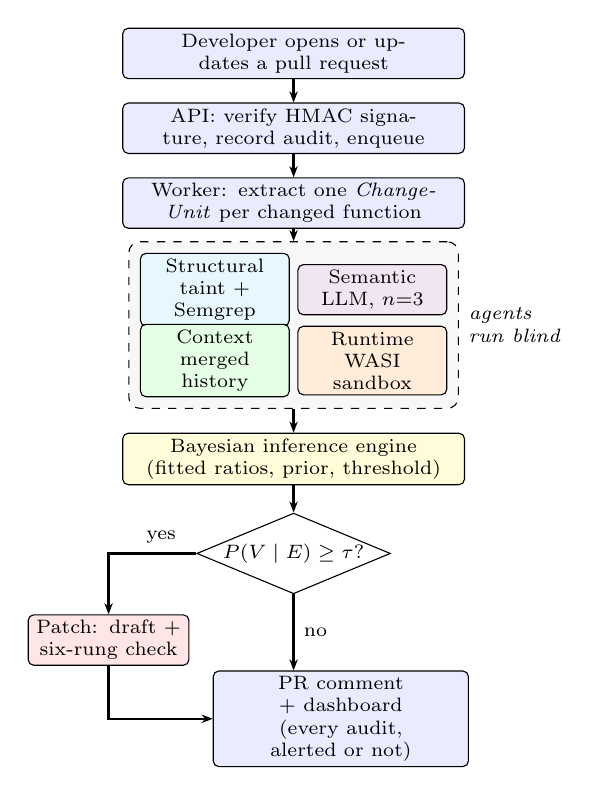
\begin{tikzpicture}[
  font=\scriptsize,
  box/.style={draw, rounded corners=2pt, align=center, minimum height=0.6cm,
              text width=#1, inner sep=2pt},
  box/.default=4.2cm,
  arr/.style={-{Stealth[length=4pt]}, thick}]
\node[box, fill=blue!8] (pr) at (0,0) {Developer opens or updates a pull request};
\node[box, fill=blue!8] (api) at (0,-0.95) {API: verify HMAC signature, record audit, enqueue};
\node[box, fill=blue!8] (ext) at (0,-1.9) {Worker: extract one \textit{ChangeUnit} per changed function};
\node[box=1.75cm, fill=cyan!10]   (s) at (-1.0,-3.0) {Structural\\taint + Semgrep};
\node[box=1.75cm, fill=violet!10] (m) at ( 1.0,-3.0) {Semantic\\LLM, $n{=}3$};
\node[box=1.75cm, fill=green!10]  (c) at (-1.0,-3.9) {Context\\merged history};
\node[box=1.75cm, fill=orange!15] (r) at ( 1.0,-3.9) {Runtime\\WASI sandbox};
\begin{scope}[on background layer]
\node[draw, dashed, rounded corners, fill=gray!6, inner sep=4pt,
      fit=(s)(m)(c)(r)] (ag) {};
\end{scope}
\node[font=\scriptsize\itshape, anchor=west, align=left] at (ag.east) {agents\\run blind};
\node[box, fill=yellow!15] (bay) at (0,-5.15) {Bayesian inference engine\\(fitted ratios, prior, threshold)};
\node[diamond, draw, aspect=2.4, inner sep=0.3pt, align=center] (dec) at (0,-6.35) {$P(V\mid E)\ge\tau$?};
\node[box=1.9cm, fill=red!10] (pat) at (-2.35,-7.45) {Patch: draft +\\six-rung check};
\node[box=3.1cm, fill=blue!8] (out) at (0.6,-8.45) {PR comment + dashboard\\(every audit, alerted or not)};
\draw[arr] (pr) -- (api);
\draw[arr] (api) -- (ext);
\draw[arr] (ext) -- (ag);
\draw[arr] (ag) -- (bay);
\draw[arr] (bay) -- (dec);
\draw[arr] (dec.west) -| node[pos=0.2, above]{yes} (pat.north);
\draw[arr] (pat.south) |- (out.west);
\draw[arr] (dec.south) -- node[right]{no} (dec.south |- out.north);
\end{tikzpicture}
\caption{Workflow of CodeSheriff. The API only verifies and queues; all
analysis happens in a separate worker. The four agents never see each
other's output.}
\label{fig:workflow}
\end{figure}

\subsection{Unit of Analysis: the Changed Function}
\label{subsec:unit}

\textit{Why:} A diff fragment is too small to reason about, and a whole
file is too large and mixes unrelated code. Also, the fused probability is
fitted on labelled functions, so production must analyse the same kind of
object.

\textit{What:} CodeSheriff analyses one \emph{ChangeUnit} per changed
function. A ChangeUnit holds the file path, the function name, the old and
new source of the function, and the list of changed lines.

\textit{How:} The worker downloads the base and head versions of each
changed file. It parses both with tree-sitter, which tolerates the syntax
errors that are common in unfinished commits, and computes the changed
lines by comparing the two versions. Each changed line is mapped to the
outermost function that contains it. Changes outside any function form a
single module-level unit, because hard-coded credentials usually live at
module level. A function that is too large for the analysis budget is not
cut short; the agents report that they could not analyse it. Truncating it
would produce confident findings from half-read code.

\subsection{The Four Agents}
\label{subsec:agents}

Every agent has exactly the same interface: it receives one ChangeUnit and
returns a list of statements. Table~\ref{tab:agents} summarises what each
agent relies on and when it is expected to fail.

\begin{table}[t]
\centering
\caption{The four agents and how each one can fail}
\label{tab:agents}
\small
\setlength{\tabcolsep}{3pt}
\begin{tabular}{p{1.5cm}p{3.0cm}p{3.0cm}}
\toprule
Agent & Basis of decision & Fails when \\
\midrule
Structural & Rule-based data-flow proof; no LLM & The bug has no syntactic pattern \\
Semantic   & Knowledge of a language model & The model invents a bug or agrees too easily \\
Context    & The repository's own merged code & The repository has no relevant history \\
Runtime    & Direct observation in a sandbox & The code cannot run in a sandbox \\
\bottomrule
\end{tabular}
\end{table}

\subsubsection{Structural Agent}
\textit{Why:} Many injection flaws follow a clear pattern: data that the
caller controls reaches a dangerous call without being cleaned. Such a
flow can be proven mechanically, without any model.

\textit{What:} The agent reports a weakness when an untrusted value can
reach a dangerous operation (a \emph{sink}), such as an SQL query, a shell
command, or a file path.

\textit{How:} It builds a definition--use graph of the function and follows
data from each function parameter to known sinks. Every parameter is
treated as untrusted, because the function signature is the trust boundary
of the unit. Each sink rule states which argument positions are dangerous;
for example, only the first argument of \texttt{cursor.execute} is
dangerous, which is how a parameterised query is correctly treated as
safe. A validating guard such as ``if the value is not in the allowed list,
raise an error'' clears the taint, while a simple ``is None'' check does
not. A second backend, Semgrep~\cite{semgrep}, runs pattern rules on the
same function. Because both backends read the same text with a similar
technique, their results are merged by taking the stronger one, and they
count as \emph{one} witness in fusion.

\subsubsection{Semantic Agent}
\textit{Why:} Some weaknesses, such as a missing authorization check, have
no fixed syntax. Finding them requires understanding what the function is
meant to do.

\textit{What:} A hosted language model is asked for the intent of the
function, its trust boundaries, and the security rule (invariant) that the
change breaks.

\textit{How:} The model is sampled three times with different seeds. The
agent's confidence is the share of samples that report the same weakness,
so a finding seen in all three samples is stronger than a finding seen in
one. Two safeguards control the known failure modes of language models.
First, the analysed code is wrapped between random markers generated for
every request, so text inside the code cannot pretend to be an instruction
(prompt injection). Second, a \emph{hallucination gate} rejects a finding
if its weakness type is out of scope, if it names a different file, if the
dangerous call it quotes does not appear word-for-word in the code, or if
its line numbers lie outside the function. Worked examples of safe code are
included in the prompt so that the model learns that ``no vulnerability''
is an acceptable answer.

\subsubsection{Context Agent}
\textit{Why:} A change can be dangerous only because of what the
repository normally does. For example, removing an ownership check from
one endpoint is a regression if all similar endpoints perform that check.

\textit{What:} The agent reports a security control that the repository's
merged code establishes and the changed function does not apply.

\textit{How:} Merged functions are stored as vector embeddings (384
dimensions, computed locally) in PostgreSQL with pgvector. For each unit,
similar merged functions of the \emph{same} repository are retrieved.
A control is accepted as a rule only if the same function applied it
before, or if at least two different sibling functions apply it; one
neighbour's habit is treated as coincidence. The agent reports only
authorization weaknesses (CWE-862 and CWE-639). This narrow scope is
deliberate: it keeps the agent from repeating what the other agents
already say.

\subsubsection{Runtime Agent}
\textit{Why:} The strongest evidence that untrusted data reaches a
dangerous operation is to see it happen. However, running untrusted
pull-request code is exactly how CI systems are attacked, so it must be
done in strict isolation.

\textit{What:} The agent executes the changed function once and reports
which dangerous operations an untrusted value actually reached.

\textit{How:} The function runs inside a WebAssembly~\cite{haas2017wasm}
sandbox built on Wasmtime~\cite{wasmtime} and the WebAssembly System
Interface (WASI), which gives software fault isolation~\cite{wahbe1993sfi}.
The sandbox has no network (a module that asks for a socket fails to load),
an empty environment, and no host files. Three limits bound each run:
instruction fuel, wall-clock time, and memory. Every
parameter receives a unique random token as its value. Because the token
is ordinary text, it survives string formatting and concatenation. If the
token appears in the argument of a dangerous call, the agent reports a
detection. If the run can only reach that call because the harness had to
answer a check it could not evaluate, the agent abstains instead of
reporting.

\subsection{Three Kinds of Agent Statements}
\label{subsec:evidence}

\textit{Why:} Most tools give a yes/no answer per agent. This hides an
important difference: an agent that \emph{looked and found nothing} has
provided evidence of safety, while an agent that \emph{could not look} has
provided no evidence at all.

\textit{What and how:} Each agent returns one of three statements for each
unit, as shown in Table~\ref{tab:evidence}. A silence also lists the
weakness types the agent is able to check, so that, for example, the
structural agent's silence does not count against an authorization flaw
it has no rules for.

\begin{table}[t]
\centering
\caption{The three kinds of statement an agent can make}
\label{tab:evidence}
\small
\setlength{\tabcolsep}{3pt}
\begin{tabular}{p{1.55cm}p{3.35cm}p{2.5cm}}
\toprule
Statement & Meaning & Effect on probability \\
\midrule
Detection  & Agent ran and found a weakness, with a score & Increases it \\
Silence    & Agent ran and found nothing  & Decreases it \\
Abstention & Agent could not run (timeout, no tool, too large) & None (factor $=1$) \\
\bottomrule
\end{tabular}
\end{table}

\subsection{Bayesian Evidence Fusion}
\label{subsec:fusion}

\textit{Why:} Majority voting treats every agent as equally reliable and
ignores how rare vulnerabilities are. Bayes' rule instead weighs each
statement by how reliable that kind of statement has been in the past, and
starts from a realistic base rate.

\textit{What:} For every candidate weakness in a unit, the engine
computes the posterior probability $P(V \mid E)$ that the change is
vulnerable $(V)$ given the statements $(E)$ of the four agents.

\textit{How:} Each agent's statement is first placed into one of four
\emph{cells}: a detection with a score of at least $0.8$ (high), between
$0.5$ and $0.8$ (medium), below $0.5$ (low), or silence. For each agent $a$
and cell $z$, a likelihood ratio (LR) states how much more often that cell
occurs for vulnerable code than for safe code:
\begin{equation}
\Lambda_a(z)=\frac{P(z \mid V)}{P(z \mid \neg V)}
\approx \frac{(k_{V}+1)/(N_{V}+m)}{(k_{S}+1)/(N_{S}+m)}
\label{eq:lr}
\end{equation}
Here $k_V$ and $k_S$ count the vulnerable and safe labelled examples that
fell into cell $z$, $N_V$ and $N_S$ are the totals, and $m$ is the number
of cells. Adding one to each count (Laplace smoothing) avoids dividing by
zero when a cell was never seen. An LR above $1$ is evidence for a
vulnerability, below $1$ is evidence against, and exactly $1$ is neutral.
Two further rules keep the ratios honest: a cell that was never observed
receives exactly $1$, and every LR is clamped to $[0.05, 20]$ so no single
agent can dominate. An abstention always receives exactly $1$.

The prior probability $\pi$ is turned into odds and multiplied by one LR
per agent:
\begin{equation}
O(V \mid E)=\frac{\pi}{1-\pi}\;\prod_{a=1}^{4}\Lambda_a(z_a)
\label{eq:odds}
\end{equation}
The odds are then converted back into a probability:
\begin{equation}
P(V \mid E)=\frac{O(V \mid E)}{1+O(V \mid E)}
\label{eq:posterior}
\end{equation}
The product in (\ref{eq:odds}) always has exactly four factors, one per
agent, whether an agent spoke or not. Because silences contribute factors
below $1$, the posterior can go down as well as up.

\textit{Worked example.} With the declared prior $\pi=0.03$, the prior odds
are $0.031$. Suppose the structural agent gives a medium detection
($\Lambda=15.56$), the semantic agent a high detection ($\Lambda=9.48$),
the context agent abstains ($\Lambda=1$), and the runtime agent gives a
high detection ($\Lambda=6.92$). The odds become
$0.031\times15.56\times9.48\times1\times6.92\approx31.6$, and the posterior
is $31.6/32.6\approx0.97$. If instead only the semantic agent had
detected and the other three had abstained, the posterior would be $0.227$,
which is exactly the fitted alert threshold. In plain words, the threshold
means: \emph{a strong semantic finding that no other agent contradicts is
just enough to alert}.

\subsection{Patch Suggestion and Verification}
\label{subsec:patch}

\textit{Why:} An alert is more useful when it comes with a fix, but an
unchecked fix produced by a language model can break the code or leave the
flaw in place.

\textit{What:} For every finding above the threshold, the patch module
drafts a repaired function, checks it against a fixed ladder of six rungs
(Table~\ref{tab:ladder}), and, if it passes, posts it as a GitHub
\emph{suggested change}. CodeSheriff never commits, pushes, or merges.

\textit{How:} The model receives the same protected prompt as the semantic
agent and returns only the repaired function. If a draft fails, the next
attempt receives the list of reasons for rejection, written by CodeSheriff,
and never the rejected draft itself, since that draft is shaped by
untrusted code. At most three drafts are tried. Every rung has three
possible outcomes: passed, failed, or not run, so a check that could not
run is never shown as passed. A verified fix is published only if all the
lines it replaces lie inside the pull request's changed lines, because
GitHub accepts suggestions only there. The repository's own test suite is
never executed, because doing so would need network and filesystem access
that the sandbox exists to deny.

\begin{table}[t]
\centering
\caption{Verification ladder for a suggested patch}
\label{tab:ladder}
\small
\setlength{\tabcolsep}{3pt}
\begin{tabular}{cp{6.9cm}}
\toprule
Rung & Check \\
\midrule
1 & The patch is valid Python (parsed, never executed) \\
2 & The function keeps the signature its callers depend on \\
3 & The patch uses no name that the file does not define or import \\
4 & The patch actually changes the function \\
5 & The structural and runtime agents that detected the weakness no longer detect it \\
6 & The same agents find no new weakness in the repaired function \\
\bottomrule
\end{tabular}
\end{table}

% =====================================================================
\section{Implementation Details} \label{IMP}
% =====================================================================

\subsection{Software Architecture}
CodeSheriff is written in Python 3.12 as a monorepo of nine packages and
three applications. Table~\ref{tab:stack} lists the main technologies. The
system runs as two separate processes with separate credentials. The API
process holds the GitHub webhook secret and the sign-in secret, and never
analyses code. The worker process holds the language-model key and runs
all agents. A task passed between them carries only an audit identifier.
An import checker in the build enforces that no agent imports another
agent, the database, or the fusion engine.

\begin{table}[t]
\centering
\caption{Implementation technology stack}
\label{tab:stack}
\small
\setlength{\tabcolsep}{3pt}
\begin{tabular}{p{2.2cm}p{5.6cm}}
\toprule
Layer & Technology \\
\midrule
API and queue   & FastAPI, Celery, Redis \\
Storage         & PostgreSQL 16, pgvector, SQLAlchemy, Alembic \\
Parsing         & tree-sitter (extraction), Python \texttt{ast} (patch check) \\
Structural      & Custom taint engine (networkx), Semgrep \\
Semantic        & Hosted Gemini Flash-Lite model, $n=3$ samples \\
Context         & Sentence-Transformers \texttt{bge-small-en-v1.5} \\
Runtime         & Wasmtime + WASI, CPython 3.12 compiled to WebAssembly \\
Dashboard       & Next.js, TypeScript, Tailwind, Recharts \\
Quality gates   & pytest (1249 tests), mypy strict, ruff, import-linter \\
\bottomrule
\end{tabular}
\end{table}

\subsection{Security of the Pipeline}
The webhook signature (HMAC-SHA256) is checked on the raw request body
before the body is parsed. Source code is kept only in memory; the
database stores findings, statements, and hashes of the source, never the
source itself. No file path chosen by the pull-request author is written
into the pull-request comment. The dashboard only reads data, and every
query is limited to the GitHub installations of the signed-in user. The
alert threshold is shown on the dashboard but cannot be changed there,
because a per-repository threshold would silently change the meaning of
past alerts.

\subsection{Labelled Dataset}
\textit{Why:} Calibration can only be measured against ground truth.
\textit{What:} A hand-written corpus of 76 Python functions arranged as 38
\emph{twin pairs}. Each pair holds the same function twice, once vulnerable
and once fixed, so a false positive on the safe twin is directly visible.
The corpus covers the ten in-scope weakness classes of the Common Weakness
Enumeration (CWE)~\cite{cwe}: path traversal (22), OS command injection
(78), cross-site scripting (79), SQL injection (89), code injection (94),
unsafe deserialization (502), insecure direct object reference (639),
hard-coded credentials (798), missing authorization (862), and
server-side request forgery (918).
\textit{How:} Pairs are assigned to three splits by pair, so the two twins
never fall into different splits (Table~\ref{tab:corpus}). The protocol is
strict: likelihood ratios are fitted only on the \emph{calibration} split,
the threshold is selected only on the \emph{validation} split, and the
\emph{test} split is evaluated exactly once, at the end. No agent can
import the corpus, so no agent can read a label.

\begin{table}[t]
\centering
\caption{Corpus composition (units per split)}
\label{tab:corpus}
\small
\setlength{\tabcolsep}{4pt}
\begin{tabular}{lcccc}
\toprule
CWE & Pairs & Calibration & Validation & Test \\
\midrule
CWE-22  & 3 & 4 & 0 & 2 \\
CWE-78  & 3 & 2 & 2 & 2 \\
CWE-79  & 3 & 4 & 0 & 2 \\
CWE-89  & 3 & 6 & 0 & 0 \\
CWE-94  & 3 & 4 & 2 & 0 \\
CWE-502 & 3 & 4 & 2 & 0 \\
CWE-639 & 6 & 6 & 2 & 4 \\
CWE-798 & 3 & 4 & 0 & 2 \\
CWE-862 & 8 & 8 & 4 & 4 \\
CWE-918 & 3 & 4 & 2 & 0 \\
\midrule
Total   & 38 & 46 & 14 & 16 \\
\bottomrule
\end{tabular}
\end{table}

\subsection{Declared Base Rate}
Because every vulnerable case has a safe twin, the corpus is half
vulnerable by construction. This does not describe real pull requests, in
which vulnerable changes are rare. The prior is therefore \emph{declared}
as $\pi=0.03$ and is not measured from the corpus. The likelihood ratios in
(\ref{eq:lr}) are conditioned on the label, so they do not depend on the
share of vulnerable cases; this is why a balanced corpus is the right shape
for fitting them. All reported metrics are weighted so that vulnerable
claims account for $3\%$ of the weight, which estimates behaviour in
production rather than on the balanced corpus.

\subsection{Experimental Environment}
Experiments were run on a machine with an Intel Core i5 processor and
16~GB RAM. The fitting and evaluation use recorded language-model
responses, so a rerun makes no network call and reproduces every number
exactly. Every fitted artifact stores a hash of the corpus and of the split
assignment it was fitted on, so a later edit to the data shows up as a stale
fit.

% =====================================================================
\section{Result Analysis and Discussion} \label{RES}
% =====================================================================

\subsection{Evaluation Metrics}
Detection quality is reported as precision (P), recall (R), and $F_1$.
Calibration is reported with two standard measures. The \emph{Brier
score}~\cite{brier1950} is the mean squared difference between the
predicted probability $p_i$ and the true label $y_i\in\{0,1\}$:
\begin{equation}
\mathrm{Brier}=\frac{1}{N}\sum_{i=1}^{N}\left(p_i-y_i\right)^2
\label{eq:brier}
\end{equation}
The \emph{Expected Calibration Error} (ECE)~\cite{guo2017calibration}
groups predictions into ten equal-width bins $B_b$ and compares the average
confidence with the observed frequency of vulnerabilities in each bin:
\begin{equation}
\mathrm{ECE}=\sum_{b=1}^{10}\frac{|B_b|}{N}\,
\bigl|\,\mathrm{freq}(B_b)-\mathrm{conf}(B_b)\,\bigr|
\label{eq:ece}
\end{equation}
For both measures, lower is better, and $0$ is perfect. A statement about
one weakness in one unit is called a \emph{claim}. The calibration split
yields $49$ claims and the validation split yields $15$ claims ($7$
vulnerable).

\subsection{Individual Agent Performance}
Before fusion, each agent was measured alone on the calibration split,
only on the cases it is designed to detect, and on all safe twins for
false positives. Table~\ref{tab:agentperf} shows that every agent reached
full recall on its own scope without a single false positive. The semantic
agent is measured differently, because a language model can fail in ways
that a rule cannot: none of its accepted findings named a sink that was
absent from the code, no injected instruction changed its answer, and it
correctly left $94\%$ of safe twins without a finding.

\begin{table}[t]
\centering
\caption{Stand-alone agent measurement (calibration split)}
\label{tab:agentperf}
\small
\setlength{\tabcolsep}{3pt}
\begin{tabular}{lccc}
\toprule
Agent & Recall on own scope & Safe twins & False positives \\
\midrule
Structural (taint) & 13/13 & 23 & 0 \\
Context            & 5/5   & 11 & 0 \\
Runtime            & 9/9   & 23 & 0 \\
\midrule
\multicolumn{4}{l}{Semantic: 0 hallucinated sinks, 0\% injection success,}\\
\multicolumn{4}{l}{\quad $94\%$ of safe twins correctly passed}\\
\bottomrule
\end{tabular}
\end{table}

\subsection{Fitted Likelihood Ratios}
Table~\ref{tab:lr} lists the likelihood ratios fitted on the calibration
split using (\ref{eq:lr}). The table can be read directly: a medium
structural detection makes a vulnerability $15.6$ times more likely, while
a structural silence makes it about $15$ times \emph{less} likely
($0.065$). Two cells behave in an interesting way. A low-scoring semantic
detection ($0.74$) and a medium-scoring one ($0.56$) are evidence of
\emph{safety}. This means that when the model reports a weakness in only
one or two of its three samples, the code was more often safe than
vulnerable. A voting system would count such a finding as a ``yes'' vote;
the fitted ratio correctly treats it as weak evidence against. Cells marked
``--'' were never observed and contribute exactly $1$.

\begin{table}[t]
\centering
\caption{Fitted likelihood ratios per agent and cell}
\label{tab:lr}
\small
\setlength{\tabcolsep}{4pt}
\begin{tabular}{lcccc}
\toprule
Agent & High & Medium & Low & Silence \\
\midrule
Structural & 2.22  & 15.56 & --   & 0.065 \\
Semantic   & 9.48  & 0.56  & 0.74 & 0.304 \\
Context    & 2.00  & 4.00  & 2.00 & 0.167 \\
Runtime    & 6.92  & --    & --   & 0.115 \\
\bottomrule
\end{tabular}
\end{table}

\subsection{Comparison with Baselines}
CodeSheriff is compared with two baselines that use the \emph{same}
agent statements, so the only difference is how the statements are
combined. \emph{Majority vote} alerts according to the share of agents
that detected, ignoring abstentions. \emph{Prior only} ignores all agents
and always predicts the $3\%$ base rate. All systems use the same threshold
of $0.227$. Table~\ref{tab:comparison} reports the results on both splits,
and Fig.~\ref{fig:compare} shows $F_1$ and Brier score on the validation
split.

\begin{table}[t]
\centering
\caption{CodeSheriff versus baselines using identical agent statements.
Best per column in bold.}
\label{tab:comparison}
\small
\setlength{\tabcolsep}{3.5pt}
\begin{tabular}{llccccc}
\toprule
Split & System & ECE$\downarrow$ & Brier$\downarrow$ & P$\uparrow$ & R$\uparrow$ & $F_1\uparrow$ \\
\midrule
Valid.
 & Prior only    & \textbf{0.000} & 0.029 & 0.000 & 0.000 & 0.000 \\
 & Majority vote & 0.141 & 0.059 & 0.076 & \textbf{1.000} & 0.142 \\
 & CodeSheriff   & 0.027 & \textbf{0.013} & \textbf{1.000} & 0.857 & \textbf{0.923} \\
\midrule
Calib.
 & Prior only    & \textbf{0.000} & 0.029 & 0.000 & 0.000 & 0.000 \\
 & Majority vote & 0.092 & 0.068 & 0.161 & \textbf{0.957} & 0.276 \\
 & CodeSheriff   & 0.009 & \textbf{0.010} & \textbf{1.000} & 0.696 & \textbf{0.821} \\
\bottomrule
\end{tabular}
\end{table}

\begin{figure}[t]
\centering
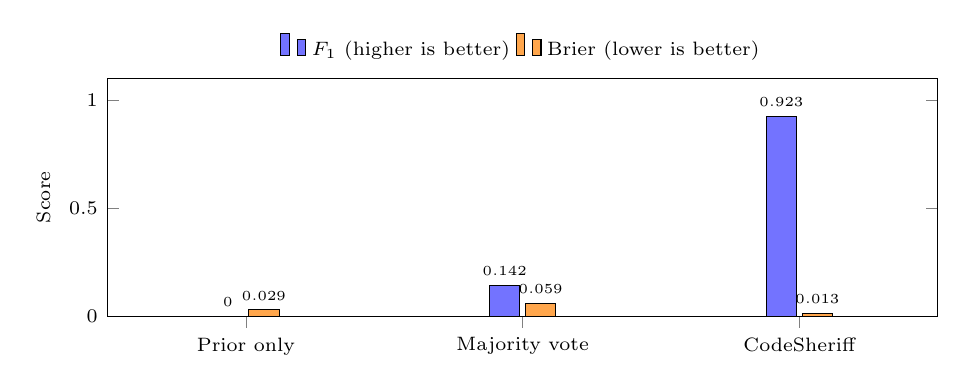
\begin{tikzpicture}
\begin{axis}[
  ybar, width=\columnwidth, height=4.6cm,
  bar width=11pt, enlarge x limits=0.25,
  ymin=0, ymax=1.1,
  symbolic x coords={Prior only,Majority vote,CodeSheriff},
  xtick=data, tick label style={font=\scriptsize},
  ylabel={Score}, ylabel style={font=\scriptsize},
  xtick pos=left, legend columns=2,
  legend style={font=\scriptsize, at={(0.5,1.03)}, anchor=south, draw=none},
  nodes near coords, nodes near coords style={font=\tiny},
  every node near coord/.append style={/pgf/number format/fixed,
                                       /pgf/number format/precision=3}]
\addplot[fill=blue!55]  coordinates {(Prior only,0) (Majority vote,0.142) (CodeSheriff,0.923)};
\addplot[fill=orange!70] coordinates {(Prior only,0.029) (Majority vote,0.059) (CodeSheriff,0.013)};
\legend{$F_1$ (higher is better), Brier (lower is better)}
\end{axis}
\end{tikzpicture}
\caption{$F_1$ and Brier score on the validation split.}
\label{fig:compare}
\end{figure}

On the validation split, CodeSheriff reaches $F_1=0.923$ with perfect
precision, alerting on $6$ of $15$ claims. Majority vote over exactly the
same statements reaches only $F_1=0.142$: it finds every vulnerability, but
most of its alerts are false, because a single agent's detection is enough
to trigger it and there is no prior to hold it back. It is also five times
worse calibrated (ECE $0.141$ versus $0.027$). The prior-only baseline
shows why ECE must not be read alone: it scores a perfect ECE of $0$ while
detecting nothing. The Brier score exposes the difference, since
CodeSheriff's $0.013$ is less than half of the prior's $0.029$. CodeSheriff
is therefore both \emph{calibrated} and \emph{useful}. The same ordering
holds on the larger calibration split.

\subsection{Reliability Diagram}
Fig.~\ref{fig:reliability} plots the average predicted probability in each
bin against the observed share of vulnerable claims on the validation
split. A perfectly calibrated system lies on the diagonal. Most claims
receive a very low probability and are indeed safe (bottom-left point,
$8$ claims). High-probability claims are all vulnerable (top-right points).
In the middle range, two bins lie above the diagonal, which means the
system was slightly \emph{under}-confident there: claims given $23\%$ and
$34\%$ were in fact vulnerable. One claim given $13\%$ was safe. These
middle bins contain only one or two claims each, so they carry very little
weight in the ECE; a larger dataset is needed to judge this region
reliably.

\begin{figure}[t]
\centering
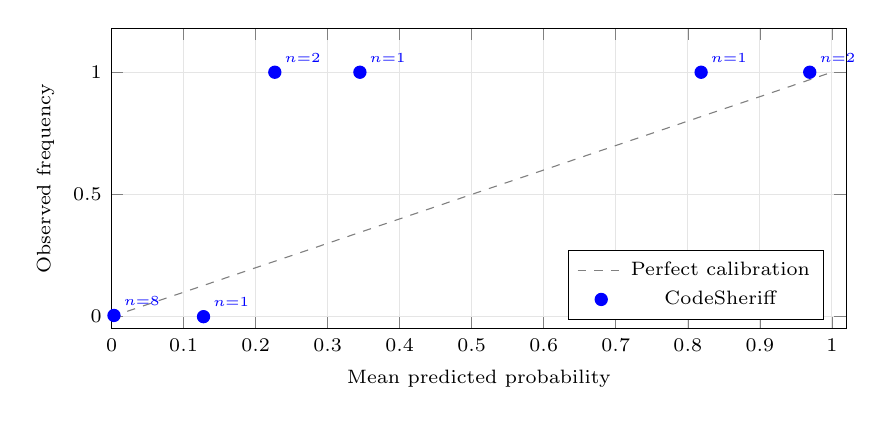
\begin{tikzpicture}
\begin{axis}[
  width=0.9\columnwidth, height=5.4cm,
  xmin=0, xmax=1.02, ymin=-0.05, ymax=1.18,
  xlabel={Mean predicted probability}, ylabel={Observed frequency},
  label style={font=\scriptsize}, tick label style={font=\scriptsize},
  legend style={font=\scriptsize, at={(0.97,0.03)}, anchor=south east},
  grid=major, grid style={gray!20}]
\addplot[dashed, gray, domain=0:1] {x};
\addplot[only marks, mark=*, blue, mark size=2.2pt,
  nodes near coords, point meta=explicit symbolic,
  every node near coord/.append style={font=\tiny, anchor=south west}]
  coordinates {
  (0.0034,0.0050) [$n{=}8$]
  (0.1277,0.0)    [$n{=}1$]
  (0.2267,1.0)    [$n{=}2$]
  (0.3448,1.0)    [$n{=}1$]
  (0.8185,1.0)    [$n{=}1$]
  (0.9693,1.0)    [$n{=}2$]};
\legend{Perfect calibration, CodeSheriff}
\end{axis}
\end{tikzpicture}
\caption{Reliability diagram on the validation split (15 claims).}
\label{fig:reliability}
\end{figure}

\subsection{Selecting the Alert Threshold}
The threshold was chosen on the validation split by sweeping every
distinct posterior value and keeping the one with the best weighted $F_1$
(Fig.~\ref{fig:threshold}). Below $0.227$, recall is complete but one safe
claim with a posterior of $0.13$ is alerted, and because safe code is far
more common in production, that single false alarm lowers precision to
$0.17$. Above $0.227$, precision stays perfect but true vulnerabilities
start to be missed. The value $0.227$ is the point where both are balanced.
Because the threshold was chosen on this split, these validation figures
are selection-time estimates and not a held-out measurement.

\begin{figure}[t]
\centering
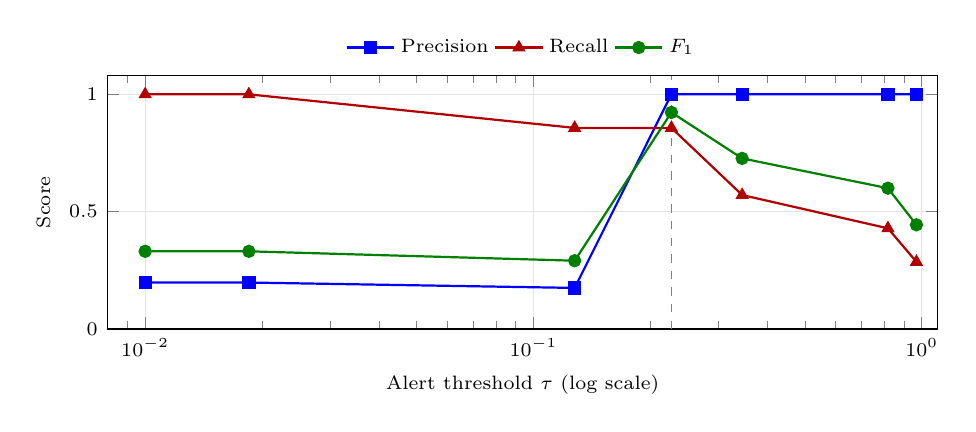
\begin{tikzpicture}
\begin{semilogxaxis}[
  width=\columnwidth, height=4.8cm,
  xmin=0.008, xmax=1.1, ymin=0, ymax=1.08,
  xlabel={Alert threshold $\tau$ (log scale)}, ylabel={Score},
  label style={font=\scriptsize}, tick label style={font=\scriptsize},
  legend style={font=\scriptsize, at={(0.5,1.03)}, anchor=south, draw=none},
  legend columns=3, grid=major, grid style={gray!20}]
\addplot[mark=square*, blue, thick] coordinates {
  (0.01,0.198) (0.0185,0.198) (0.1277,0.175) (0.2267,1.0) (0.3448,1.0) (0.8185,1.0) (0.9693,1.0)};
\addplot[mark=triangle*, red!70!black, thick] coordinates {
  (0.01,1.0) (0.0185,1.0) (0.1277,0.857) (0.2267,0.857) (0.3448,0.571) (0.8185,0.429) (0.9693,0.286)};
\addplot[mark=*, green!50!black, thick] coordinates {
  (0.01,0.331) (0.0185,0.331) (0.1277,0.291) (0.2267,0.923) (0.3448,0.727) (0.8185,0.600) (0.9693,0.444)};
\draw[dashed, gray] (axis cs:0.2267,0) -- (axis cs:0.2267,1.08);
\legend{Precision, Recall, $F_1$}
\end{semilogxaxis}
\end{tikzpicture}
\caption{Precision, recall and $F_1$ against the alert threshold on the
validation split. The dashed line marks the selected $\tau=0.227$.}
\label{fig:threshold}
\end{figure}

\subsection{Ablation Study}
To see what each agent contributes, one agent at a time is removed. A
removed agent is treated as an abstention, so it contributes a factor of
exactly $1$. Table~\ref{tab:ablation} and Fig.~\ref{fig:ablation} show the
results on both splits.

\begin{table}[t]
\centering
\caption{Leave-one-agent-out ablation at $\tau=0.227$}
\label{tab:ablation}
\small
\setlength{\tabcolsep}{3pt}
\begin{tabular}{lcccccc}
\toprule
 & \multicolumn{3}{c}{Validation} & \multicolumn{3}{c}{Calibration} \\
\cmidrule(lr){2-4}\cmidrule(lr){5-7}
Configuration & P & R & $F_1$ & P & R & $F_1$ \\
\midrule
Full model       & 1.000 & 0.857 & \textbf{0.923} & 1.000 & 0.696 & \textbf{0.821} \\
$-$ Structural   & 1.000 & 0.714 & 0.833 & 0.359 & 0.696 & 0.473 \\
$-$ Semantic     & 0.096 & 0.429 & 0.157 & 1.000 & 0.609 & 0.757 \\
$-$ Context      & 1.000 & 0.857 & 0.923 & 1.000 & 0.696 & 0.821 \\
$-$ Runtime      & 1.000 & 0.857 & 0.923 & 1.000 & 0.696 & 0.821 \\
\bottomrule
\end{tabular}
\end{table}

\begin{figure}[t]
\centering
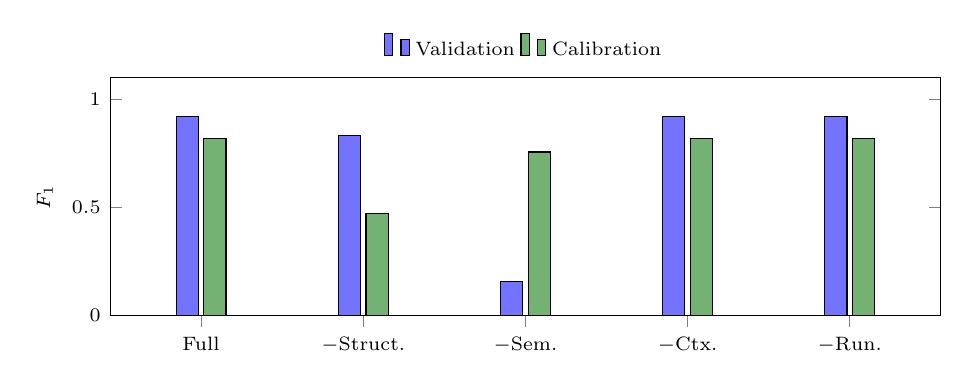
\begin{tikzpicture}
\begin{axis}[
  ybar, width=\columnwidth, height=4.6cm,
  bar width=8pt, enlarge x limits=0.14,
  ymin=0, ymax=1.1,
  symbolic x coords={Full,$-$Struct.,$-$Sem.,$-$Ctx.,$-$Run.},
  xtick=data, tick label style={font=\scriptsize},
  ylabel={$F_1$}, ylabel style={font=\scriptsize},
  xtick pos=left, legend columns=2,
  legend style={font=\scriptsize, at={(0.5,1.03)}, anchor=south, draw=none}]
\addplot[fill=blue!55] coordinates {(Full,0.923) ($-$Struct.,0.833) ($-$Sem.,0.157) ($-$Ctx.,0.923) ($-$Run.,0.923)};
\addplot[fill=green!45!black!55] coordinates {(Full,0.821) ($-$Struct.,0.473) ($-$Sem.,0.757) ($-$Ctx.,0.821) ($-$Run.,0.821)};
\legend{Validation, Calibration}
\end{axis}
\end{tikzpicture}
\caption{$F_1$ after removing one agent at a time.}
\label{fig:ablation}
\end{figure}

The two splits disagree about which agent matters most, and this
disagreement is itself the main finding. On the validation split, removing
the semantic agent collapses $F_1$ from $0.923$ to $0.157$. On the
calibration split, removing the structural agent causes the largest drop,
from $0.821$ to $0.473$, because precision falls to $0.359$. No single
agent is sufficient on both splits, which supports the use of
heterogeneous agents. Removing the context or the runtime agent does not
change the final decisions on either split. This is reported as a null
result and not as proof that these agents are redundant: both agents have
narrow scopes (the context agent covers two CWEs), so their evidence
usually confirms a decision that another agent has already made. They
still move the posterior; for example, removing the runtime agent raises
the calibration-split ECE from $0.009$ to $0.011$.

\subsection{Qualitative Comparison with Related Work}
A direct numerical comparison with published systems is not meaningful,
because they are evaluated on different languages, weakness sets and
metrics. Table~\ref{tab:related} therefore compares capabilities. To our
knowledge, CodeSheriff is the first of these systems to combine
heterogeneous agents with a calibrated probability, sandboxed execution,
and verified patch suggestions inside the pull-request workflow.

\begin{table}[t]
\centering
\caption{Capability comparison with related systems
(\cmark: reported; --: not reported in the cited work)}
\label{tab:related}
\small
\setlength{\tabcolsep}{2.5pt}
\begin{tabular}{lccccc}
\toprule
Capability & \cite{ref2} & \cite{ref1} & \cite{ref16} & \cite{ref6} & Ours \\
\midrule
Multiple agents              & --     & --     & \cmark & \cmark & \cmark \\
Distinct technique per agent & --     & --     & --     & --     & \cmark \\
Calibrated confidence        & \cmark & --     & --     & --     & \cmark \\
Repository context           & --     & \cmark & \cmark & --     & \cmark \\
Sandboxed execution          & --     & --     & --     & --     & \cmark \\
Verified patches             & --     & --     & --     & --     & \cmark \\
PR integration               & --     & --     & --     & --     & \cmark \\
\bottomrule
\end{tabular}
\end{table}

\subsection{Limitations}
The results should be read with the following limits in mind. First, the
corpus is small, written by the authors, Python-only, and limited to ten
CWEs, so the figures describe this corpus and not arbitrary pull requests.
The validation split has only $15$ claims, which is too few to attach a
useful confidence interval. Second, the held-out test split has not yet
been evaluated; it is reserved for a single final run. Third, Semgrep has
no build for the Windows machine used for fitting, so the structural
ratios describe the taint engine alone; a Linux image with all four agents
active has been prepared for the final run. Fourth, the $3\%$ base rate is
declared, not measured, and every weighted figure scales with it. Finally,
external tools such as Semgrep, Bandit and a single-pass language model
have not yet been scored under the same protocol.

% =====================================================================
\section{Conclusion and Future Scope} \label{CON}
% =====================================================================

This paper presented CodeSheriff, a security auditor for GitHub pull
requests in which four agents, based on four different techniques, analyse
each changed function independently, and a Bayesian engine combines their
statements into a calibrated probability. The design separates an agent
that found nothing from an agent that could not look, fits every
likelihood ratio and the threshold on labelled data, and never lets one
agent see another's output. On the validation split, CodeSheriff achieved
an $F_1$ of $0.923$ with perfect precision and an expected calibration
error of $0.027$, while majority voting over the identical agent
statements reached only $0.142$ and was five times worse calibrated. The
ablation study showed that no single agent is sufficient on both data
splits. Alerts are accompanied by patch suggestions that pass a fixed
six-step verification ladder and are never committed automatically.

Several directions remain for future work:
\begin{itemize}
\item Evaluate the held-out test split exactly once, on the Linux image in
which all four agents, including Semgrep, are active, after re-fitting the
structural ratios there.
\item Score Semgrep, Bandit and a single-pass language model under the same
weighted protocol, to complete the external comparison.
\item Enlarge the corpus with real vulnerability-fixing commits, so that
confidence intervals and a sensitivity analysis over the base rate and
threshold become meaningful.
\item Extend support beyond Python to JavaScript and TypeScript, which the
tree-sitter based extraction already allows.
\item Use the same sandbox to release CI/CD secrets only to verified code,
and measure the acceptance rate of suggested patches by developers.
\end{itemize}

\addcontentsline{toc}{section}{References}
\bibliographystyle{IEEEtran}
\bibliography{references}

\end{document}
